\documentclass{article}

\usepackage{fancyhdr}
\usepackage{extramarks}
\usepackage{amsmath}
\usepackage{amsthm}
\usepackage{amsfonts}
\usepackage{tikz}
\usepackage{listings}
%\usepackage[plain]{algorithm}
\usepackage{algpseudocode}
\usepackage{enumerate}
\usepackage{tikz}
\usepackage{xifthen}
\usepackage{xparse}
\usepackage{amsmath, amssymb}
\usepackage{lipsum}
\usepackage[lined,boxed,commentsnumbered]{algorithm2e}
\usepackage{endnotes}

\usetikzlibrary{automata,positioning}

%
% Basic Document Settings
%  

\topmargin=-0.45in
\evensidemargin=0in
\oddsidemargin=0in
\textwidth=6.5in
\textheight=9.0in
\headsep=0.25in

\linespread{1.1}

\pagestyle{fancy}
\lhead{\hmwkAuthorName}
\chead{\hmwkClass: \hmwkTitle}
\rhead{\firstxmark}
\lfoot{\lastxmark}
\cfoot{\thepage}

\renewcommand\headrulewidth{0.4pt}
\renewcommand\footrulewidth{0.4pt}

\setlength\parindent{0pt}

%
% Create Problem Sections
%

\newcommand{\enterProblemHeader}[1]{
    \nobreak\extramarks{}{Problem \arabic{#1} continued on next page\ldots}\nobreak{}
    \nobreak\extramarks{Problem \arabic{#1} (continued)}{Problem \arabic{#1} continued on next page\ldots}\nobreak{}
}

\newcommand{\exitProblemHeader}[1]{
    \nobreak\extramarks{Problem \arabic{#1} (continued)}{Problem \arabic{#1} continued on next page\ldots}\nobreak{}
    \stepcounter{#1}
    \nobreak\extramarks{Problem \arabic{#1}}{}\nobreak{}
}

\newcommand*\circled[1]{\tikz[baseline=(char.base)]{
		\node[shape=circle,draw,inner sep=2pt] (char) {#1};}}


\setcounter{secnumdepth}{0}
\newcounter{partCounter}
\newcounter{homeworkProblemCounter}
\setcounter{homeworkProblemCounter}{1}
\nobreak\extramarks{Problem \arabic{homeworkProblemCounter}}{}\nobreak{}

%
% Homework Problem Environment
%
% This environment takes an optional argument. When given, it will adjust the
% problem counter. This is useful for when the problems given for your
% assignment aren't sequential. See the last 3 problems of this template for an
% example.
%

\NewDocumentEnvironment{homeworkProblem}{s m}{
    \IfBooleanT{#1}{\newpage}
    \section{Problem \arabic{homeworkProblemCounter} {\small (#2)}}
    \setcounter{partCounter}{1}
    \enterProblemHeader{homeworkProblemCounter}

}{
    \exitProblemHeader{homeworkProblemCounter}
}

%
% Homework Details
%   - Title
%   - Due date
%   - Class
%   - Instructor
%   - Class number
%   - Name
%   - Student ID

\newcommand{\hmwkTitle}{Final Project}
\newcommand{\hmwkDueDate}{January 16, 2023}
\newcommand{\hmwkClass}{Probability and Mathematical Statistics}
\newcommand{\hmwkClassInstructor}{Professor Ziyu Shao}

%\newcommand{\hmwkClassID}{}

\newcommand{\hmwkAuthorName}{Ren Hui, Wanchen Su}
\newcommand{\hmwkAuthorID}{2021533089, 2021533067}

%
% Title Page
%

\title{
    \vspace{2in}
    \textmd{\textbf{\hmwkClass:\\  \hmwkTitle}}\\
    \normalsize\vspace{0.1in}\small{Due\ on\ \hmwkDueDate\ at 18:00am}\\
   %\vspace{2in}\Huge{\hmwkClassID}\\   
   \vspace{2in}
}

\author{
	Name: \textbf{\hmwkAuthorName} \\
	Student ID: \hmwkAuthorID}
\date{}


\renewcommand{\part}[1]{\textbf{\large Part (\alph{partCounter})}\stepcounter{partCounter}\\}

%
% Various Helper Commands
%

% Useful for algorithms
\newcommand{\alg}[1]{\textsc{\bfseries \footnotesize #1}}
% For derivatives
\newcommand{\deriv}[1]{\frac{\mathrm{d}}{\mathrm{d}x} (#1)}
% For partial derivatives
\newcommand{\pderiv}[2]{\frac{\partial}{\partial #1} (#2)}
% Integral dx
\newcommand{\dx}{\mathrm{d}x}
% Alias for the Solution section header
\newcommand{\solution}{\textbf{\Large Solution}}
% Probability commands: Expectation, Variance, Covariance, Bias
\newcommand{\E}{\mathrm{E}}
\newcommand{\Var}{\mathrm{Var}}
\newcommand{\Cov}{\mathrm{Cov}}
\newcommand{\Bias}{\mathrm{Bias}}

\begin{document}

\maketitle
\pagebreak

% Problem 1
\begin{homeworkProblem}*{Part 1: classical Bandit Algorithms}
    \solution
    \begin{enumerate}
        \item[1,2.]
        All simulation and results in part 1 will be in jupyter notebook part1.ipynb.
        \item[3.]
        According to python simulation, the results are:\\
        \textbf{results for $\epsilon$-greedy:}\\
        \begin{tabular}[t]{|c|c|c|c|}
        \hline
         & $\epsilon$ = 0.1 & $\epsilon$ = 0.5 & $\epsilon$ = 0.9 \\
        \hline
        reward & 3415.895 & 3083.32 & 2748.985 \\
        \hline
        $\hat{\theta}$ & $[0.699565\ 0.501675\ 0.398460]$ & $[0.700644\ 0.496887\ 0.398588]$ & $[0.700090\ 0.499850\ 0.398113]$ \\
        \hline
        \end{tabular}\\

        \textbf{results for UCB:}\\
        \begin{tabular}[t]{|c|c|c|c|}
        \hline
         & c = 0.1 & c = 0.5 & c = 0.9 \\
        \hline
        reward & 3410.44 & 2974.035 & 2824.62 \\
        \hline
        $\hat{\theta}$ & $[0.700882\ 0.492749\ 0.384489]$ & $[0.700674\ 0.499007\ 0.398861]$ & $[0.701356\ 0.498778\ 0.400231]$ \\
        \hline
        \end{tabular}\\

        \textbf{results for TS:}\\
        \begin{tabular}[t]{|c|c|c|}
        \hline
         & a,b = [[1, 1], [1, 1], [1, 1]] & a,b = [[601, 401], [401, 601], [2, 3]]\\
        \hline
        reward & 3481.33 & 3490.945 \\
        \hline
        $\hat{\theta}$ & $[0.6995964\ 0.45887541\ 0.37554019]$ & $[0.68296885\ 0.4001996\ 0.362563]$ \\
        \hline
        \end{tabular}\\

        \item[4.]
        Oracle value:$$E(r) = 5000\times0.7 = 3500$$
        \textbf{gap of $\epsilon$-greedy:}\\
        \begin{tabular}[t]{|c|c|c|c|}
        \hline
         & $\epsilon$ = 0.1 & $\epsilon$ = 0.5 & $\epsilon$ = 0.9 \\
        \hline
        reward & 3415.895 & 3083.32 & 2748.985 \\
        \hline
        gap & 84.105 & 416.68 & 751.015 \\
        \hline
        \end{tabular}\\

        \textbf{gap of UCB:}\\
        \begin{tabular}[t]{|c|c|c|c|}
        \hline
         & c = 0.1 & c = 0.5 & c = 0.9 \\
        \hline
        reward & 3410.44 & 2974.035 & 2824.62 \\
        \hline
        gap & 89.56 & 525.965 & 675.38 \\
        \hline
        \end{tabular}\\

        \textbf{gap of TS:}\\
        \begin{tabular}[t]{|c|c|c|}
        \hline
         & a,b = [[1, 1], [1, 1], [1, 1]] & a,b = [[601, 401], [401, 601], [2, 3]]\\
        \hline
        reward & 3481.33 & 3490.945 \\
        \hline
        gap & 18.67 & 9.905 \\
        \hline
        \end{tabular}\\

        As is shown above, with the given parameters, TS Algorithm is the best.\\
        
        In the $\epsilon$-greedy algorithm, $\epsilon$ decides the probability of choosing the max estimate of all the arms or choosing a random arm.
        Which means the larger $\epsilon$ is, the more evenly spread are the tests.\\
        In the UCB algorithm, the parameter c balances the estimation of $\theta_j$, and considers the number of trials on that arm.
        Increasing c means considering more about the number of test on that arm, which will allow the decision maker(DM) choose some of the less experimented arms.
        This helps in instances where the number of tests on a arm is quite small and therefore the $\theta$ of that arm is way less than it should be.\\
        If the initial value of $\alpha_j,\beta_j$ we passed in is too small,
        then the result of the first few tests may influence the final result greatly,
        and  only a few dozen tests are on the second and third arm. If this happens, the estimate value of $\theta$ will be rather inaccurate. 
        At the same time, the aggregated reward will be quite large because the DM spent very little time exploring.
        On the other hand, if the initial value of $\alpha_j,\beta_j$ we passed in is relatively large, this value of a and b may influence the final result greatly.
        As in the trial with parameter [[601, 401], [401, 601], [2, 3]], we can see that the final estimation of arm two is very close to $\frac{401}{401+601}$.
        In this case, the parameter we passed in is correct in which is the arm with the largest oracle value, so the aggregated reward is quite large.
        However, if the parameter passed in is contradictory to the actual oracle, it will take quite a long time to adjust. Consequently the aggregated reward is smaller.\\
        More impacts of $\epsilon$, c and $\alpha_j,\beta_j$ concerning exploration-exploitation will be discussed in 5.
        \item[5.]
        In the case of all algorithms, more exploitation means that we choose to pull the arm that has the greatest current estimation more often. So if the estimate of each arm differs too much from the oracle value,
        or the arm we think yield the best probability is not really the best,
        after all tests, the total aggregated reward becomes smaller. More exploration means
        the estimated value of the reward of each arm is more accurate, it helps the decision maker choose the arm better, but the exploration means that the rewards during exploration could be less.\\
        For the $\epsilon$-greedy algorithm, the larger $\epsilon$ is, there is more chance of exploration than exploitation.
        So while $\epsilon$ grows, the gaps between the algorithm estimate and the oracle value decreases, but the sum of the reward of all trials is smaller because the DM spent too much time exploring when it is not that necessary.\\
        As for the UCB Algorithm, the exploration-exploitation trade-off depends on the value of c.
        Similar to the $\epsilon$-greedy algorithm, the larger c is, there is more exploration and less exploitation.
        As can be deduced from the data in the python simulation, for larger c, the estimated value for the third arm is more accurate.
        This means that there are more times when the decision maker doesn't choose the current best arm. Consequently, the aggregated rewards over N time slots are less.\\
        The TS Algorithm is rather different from the previous ones. Its exploration is based on the beta distribution. 
        In each round, the theta of each arm is generated by a beta distribution, with means of $\frac{a}{a+b}$. So there is a chance that an arm with large means will get a smaller theta in that round. This will result in exploration.
        But that probability becomes smaller as rounds goes, so arms with small oracle values will end up being pulled only a few times.
        Which makes the estimate value of arms 2 and 3 rather inaccurate. But with the current parameters, the aggregated reward gained over the N trials should be the largest of all the algorithms. 
        TS performs best in this case because the parameters a and b we passed in corresponds with the real oracle value. On the other hand, 
        if the parameters passed in is inaccurate, it could have a large influence on the aggregated reward. For example, if we passed in [[401, 601], [601, 401], [2, 3]], it will be very hard for the algorithm to change its false knowledge that arm 2 is the best arm. This is a defect for having too little exploration.\\
        The given parameters in the question cannot fully show the trade-off between exploration and exploitation. With the given parameters, it may seem that more exploitation is always better. So the following test with actual theta as [0.5,0.7,0.9] shows that exploration is also important:\\
        \textbf{exploration-exploitation trade-off of bandit algorithms:}\\
        \begin{tabular}[t]{|c|c|c|c|}
        \hline
        $\epsilon$-greedy & parameter & $\epsilon$ = 0.005 & $\epsilon$ = 0.1  \\
        \hline
         & reward & 4213.31 & 4388.64  \\
        \hline
        UCB & parameter & c = 0.1 & c = 1  \\
        \hline
         & reward & 4358.77 & 4415.93  \\
        \hline
        TS & parameter & [[701, 301], [601, 401], [2, 3]] & [1, 1], [1, 1], [1, 1]  \\
        \hline
         & reward & 4481.905 & 4490.565  \\
        \hline
        \end{tabular}\\
        
        \item[6.]
        At first, we tried the method in \textsl{Multi-Armed Bandits with Dependent Arms}\cite{ref2}, which used clusters to process dependency, but we found its performance is not very good.
        So We mainly referred to \textsl{Multi-Armed Bandits with Correlated Arms}\cite{ref3}to improve the classical bandit algorithms under dependent cases.
        So our final version is as below:

        \begin{enumerate}[a.]
            \item Background introduction:
            First we should define the meaning of "dependency" in Bandit problem, i.e. if arm k and l are dependent, if we pull an arm k and get a reward r, we will know some information about the expected reward of l. This corresponds to real-time context such as movie recommendation. For example, when a user rated low scores for thrillers, it is reasonable to infer that he will also give a low score for horror movies which is a genre similar to thrillers. The same can be deduced for other movie genres. Here a genre is a arm, at each time slot a movie under this genre is recommended to a user, and the user's rating is the reward of the arm. Our aim is to use this dependent information and converge to the user's favourite types of movie as fast as possible, i.e. the highest reward arm. Dependent Bandit problem can also be applied to many fields like medicine test. We assume the dependent information between arms is acquired from professional knowledge or past experiments. This information will give out a expectation upper bound of other arms when pulling an arm and get a reward, which has the effect of reducing unnecessary explorations thus speeding up convergence. This will be introduced further in following parts.
            
            \item Dependency:
            Our general aim is to know which arm has the highest expectation reward, then we can always choose this arm to pull. We donate the reward of arm l as $R_l$. To know $E(R_l)$, we seek to know $E(R_l| R_k=r)$ first, which means the conditional expectation reward of an arm l given that we have received an reward r at another arm k.
            To know this information approximately, we first use the definition of "pseudo-rewards",which is a upper bound of the conditional expectation as the referred paper introduced: $$E[R_l|R_k = r]\leqslant s_{l,k}(r)$$\cite{ref3}  without loss of generality, we define $s_{l,l}(r)=r$.
            This is a $n\times n$ function matrix where n means the arm numbers. this value can be obtained from "either domain/expert knowledge or from controlled survey"\cite{ref3}. For example, it can be obtained from proportion of ingredients in medicine for medicine tests. For movie recommendation, this information can also be obtained from prior-data/surveys. For example, $s_{l,k}(r)$ can be know from the expectation of when the movie genre k is rated r, what the same user group rate for genre l. This should be an upper-bound in case of becoming misleading information. As the writer introduced, when the data-set is large, its empirical estimate can be used directly. But when it is small, we can set $s_{2,1}(0)=\hat{\mu}_{2,1}(0)+\hat{\sigma}_{2,1}(0)$. What's more, if it is hard for us to know some entries in pseudo-rewards table, we can just set it as the max possible reward. When all entries are set as max reward, the problem will be degenerate to independent case. 
            Then we define $\phi_{l,k} = E[s_{l,k}(R_k)]$ for competitive set obtaining.

            \item Data set:
            In real life, we can use several medicine for the same patient, where one medicine relates to an arm and the same patient relates to a time slot in Bandit problem. Thus we can learn the dependent relationship from experimental data through controlling variable. However, in the initial bandit problem, to obtain this data, multiple arms need to be pulled at the same time, which is not an allowed procedure. So the first thing to do before testing the algorithm performance, we generate samples of arms from their oracle possibilities and just align them by time slot to simulate pulling multiple arms in the same time slot.
            
            Next, besides using computer generated data, for real data test, we use the movie rating data-sets from grouplens.org. We give different genres serial numbers and take them as arms, while the ratings given by users are their reward, and the rating by same user group as same time slot. Finally we organize them in a csv file. 
            So each time, we choose a movie to recommend, and use reward information and dependent information to optimize our choose, to find the suitable genre movies to recommend. We did tests on the three movie scenario to match the three arm bandit problem and on the 18 movie scenario to simulate what is closer to real life data.

            What's more, each of the data has both train and test data parts. Train data is to get the pseudo-reward table and simulation is done on the test data.
            
            \item Performance evaluation:
            To make the result more clear, we use expected regret ($E[Reg(T)]$) to analyze the performance of our algorithm.
            The regret of an algorithm is defined as the difference between the cumulative reward of a genie policy, that always pulls the optimal arm, and the cumulative reward obtained by the actual algorithm over T rounds.
            So obviously its expectation in each round is the difference between the mean reward of the best arm and the mean reward of the chosen arm.
            We drew the cumulative regret of each round on a plot to visualize the performance of each algorithm.\\

            
            \item Dependent bandit algorithm:
            The dependent bandit algorithm is general that can be apply to any normal bandit algorithm. We applied it to both UCB and TS(generalized to Gauss version) algorithm there.\\
            The basic idea is to use dependency to eliminate some of the less competitive arms, so there are less choice each round, and the choices are closer to the best choice. Notice that the competitive arms may change each time.\\
            \textbf{Step 1: Identify the set of significant arms} The set of significant arms at round t $S_t$ is defined to be the set of arms that have at least $t/arms$ samples.
            In other words, $S_t$ is the set of arms that have relatively large number of samples. So we will use the data of these arms to eliminate less competitive arms by dependency. This operation is because pseudo-rewards with few sample will have larger noise, which may in-turn lead to elimination of the optimal arm. This ensure the non-competitive arms are pulled only O(1) times. \\
            \textbf{Step 2: Identify the set of competitive arms} First, find the largest estimated theta(empirical) value so far in $S_t$. Let that arm or the few arms that have the best theta be $C_t$ Then, for each arm l, find the smallest $\phi_{l,k}$ with $k\in S_t$.
            If this value is less than the largest estimated theta value so far, then this arm l is not competitive. Note that the $\phi$ value changes at each round so arm l is not eliminated forever.
            Denote the set of all competitive arms to be $A_t$\\
            \textbf{Step 3: Use bandit algorithm on $A_t\cup C_t$} According to the steps above, $A_t\cup C_t$ is the set of all competitive arms at round t.\\
            \textbf{Step 4:After pull} After pull the chosen arm k, we get a reward r(sampled from test data since dependent relation should be consistent.), then we will go to the pseudo-reward table(got when from processing train data before) to update the empirical pseudo-reward of k contributed to other arms. Other things like estimated theta, count will also be updated.

        \end{enumerate}
        The specific algorithm we used is shown below. UCB index here is $\theta+c\cdot \sqrt{\frac{2log(t)}{count}}$ for each arm, as we known\\
        \begin{algorithm}[H]
            \SetAlgoLined
            Input: pseudo-rewards $s_{l,k}(r)$\\
            Initialize: $count[k] = 0, theta[k] =0, UCB\_index=\infty $ for all k in arms\\
            \For {each round t}{
                Find $S_t$, the arm(s) that have been pulled significant times till the t-1 round.\\
                Define $k^{emp}(t) = argmax_{k\in S_t}\theta_k(t)$\\
                Initialize the competitive set $A_t$ as an empty set.\\
                \For {$k \in arms$}{
                    \If{$min_{l\in S_t}\phi_{k,l}(t)\geqslant \theta_{k^{emp}(t)}$}{
                        add arm k to $A_t$
                    }
                }
                Apply UCB to $A_t\cup {k^{emp}(t)}$\\
                Receive reward and update reward, count[k], theta[k],ucb index, empirical pseudo-reward.
            }
            \caption{Dependent UCB}
          \end{algorithm}
          The dependent TS algorithm used similar method as the dependent UCB algorithm. But since in the context of movie rating the reward is not either 0 or 1(it can be from 1 to 5), the TS algorithm cannot continue to use beta priors. So we implemented TS with gaussian priors as below:\\
          \begin{algorithm}[H]
            \SetAlgoLined
            Initialize: For each arm i, set $count_i = 0, \theta_i = \frac{min + max}{2}$\\
            \For {each round t}{
                \For {each arm i}{
                    sample $\mu_i(t)$ independently from the $N(\theta_i, \frac{beta}{count_{i(t)}+1})$ distribution.
                }
                play arm $i(t) = argmax_{i\in arms} \mu_i(t)$ and observe reward $r_t$.
                update reward, $\theta_{i(t)}$, $count_{i(t)}$
            }
            \caption{TS-gauss\cite{ref4}}
          \end{algorithm}
          The beta here is hyper parameter which we define as the half length of reward interval so that the Gauss sampling can cover the whole interval at first since initial theta is on the mid-point.
          
          The corresponding dependent TS-gauss is:\\
          \begin{algorithm}[H]
            \SetAlgoLined
            Input: pseudo-rewards $s_{l,k}(r)$\\
            Initialize: $count[k] = 0, theta[k] = \frac{min + max}{2} $ for all k in arms\\
            \For {each round t}{
                Find $S_t$, the arm(s) that have been pulled significant times till the t-1 round.\\
                Define $k^{emp}(t) = argmax_{k\in S_t}\theta_k(t)$\\
                Initialize the competitive set $A_t$ as an empty set.\\
                \For {$k \in arms$}{
                    \If{$min_{l\in S_t}\phi_{k,l}(t)\geqslant \theta_{k^{emp}(t)}$}{
                        add arm k to $A_t$
                    }
                }
                Apply TS-gauss to $A_t\cup {k^{emp}(t)}$\\
                play arm i(t) and observe reward $r_t$.
                update reward, $\theta_{i(t)}$, $count_{i(t)}$, empirical pseudo-reward.
            }
            \caption{Dependent TS-gauss}
          \end{algorithm}
          The following is the cumulative regret of the three tests, respectively on computer generated data, 3 movie data, and 18 movie data.
          \begin{figure}[htp]
            \centering
            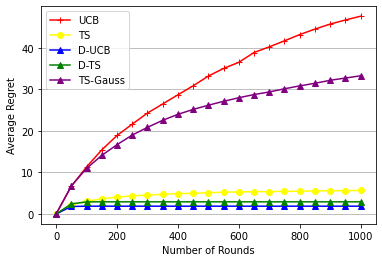
\includegraphics[width = 0.6\textwidth]{part1.png}
            \caption{The cumulative regret of UCB, Dependent UCB, TS, gaussian TS, and Dependent TS on computer generated data.(random with 0.7,0.5,0.4 probability, and align them together)}
            \label{fig1}
        \end{figure}
        \begin{figure}[htp]
            \centering
            \includegraphics[width = 0.6\textwidth]{output_3_movie.png}
            \caption{The cumulative regret of UCB, Dependent UCB, TS, gaussian TS, and Dependent TS, with three movie genres as the three arms. This data-set comes from grouplens.org}
            \label{fig2}
        \end{figure}
        \begin{figure}[htp]
            \centering
            \includegraphics[width = 0.6\textwidth]{output_18_movie.png}
            \caption{The cumulative regret of UCB, Dependent UCB, TS, gaussian TS, and Dependent TS, with 18 movie genres, as is closer to real life senerios. This data-set comes from grouplens.org}
            \label{fig3}
        \end{figure}\\
        
        As can be seen, in each of the figures, the regret of dependent TS(gauss) and dependent UCB are both better than their independent version, indicating that their perfromance is better.
    \end{enumerate}
\end{homeworkProblem}
\pagebreak
\pagebreak

\begin{homeworkProblem}*{Part 2: Bayesian Bandit Algorithms}
    \solution
    \begin{enumerate}[1.]
        \item
        See jupyter notebook for the simulation process, each time we just pull the arm of largest expected value. And when the two expected value is the same, we just take random of them. We simulated with the oracle value, Let $r(n)$ be the reward over n pulls. :\\
        \textbf{simulations:}\\
        \begin{tabular}[t]{|c|c|c|c|c|}
        \hline
        parameter & $\theta_1$ & $\theta_2$ & $\lambda$ & r(25) \\
        \hline
        test 1 & 0.7 & 0.3 & 0.9 & 5.691589689799864 \\
        \hline
        test 2 & 0.4 & 0.5 & 0.9 & 4.270186268467624 \\
        \hline
        test 3 & 0.1 & 0.3 & 0.9 & 2.180985674659367 \\
        \hline
        \end{tabular}\\
        \item
        Example for not optimal: If both $\theta_1$ and $\theta_2$ are relatively large, then we could end up with always pulling the first arm that succeeded.
        For example, if $\theta_1 = 0.8$, $\theta_2 = 0.9$, and the first arm we pulled is the first one, then there is a large possibility that the DM(Decision Maker) will always pull arm 1 because if it receives an reward in the first round, then expected probability is raised, then in round 2 DM will again pull arm 1, etc. The actual best arm (arm2), on the other hand, will always stay as the initial estimated probability of 0.5, and never get pulled, to a large probability.\\
        We used 0.8 and 0.9 as the oracle value and asked the python simulation to print out the arm it chooses each time, and it shows clearly that it almost always sticks with the arm it chose in the first round.
        In fact, as it turns out, if both arms have more than 50\% chance of yielding a reward, this policy tend to not behave that well.

        For more clear example, please see e part and the Figure, in which it is compared with the optimal policy. The differences can be seen clearly.
        \item
        Definition for "optimal policy":\\
        The optimal policy should be the one that always fully exploit the information obtained during pulling. So that given the historical results, we will calculate the expected reward for each arms and always pull the arm that has the largest expect reward.\\
        Story proof:\\
        Let us be the decision maker(DM) of a two-armed bandit problem. Presume that the experiment lasts forever, 
        but the reward returned each time is reduced by multiplying $\lambda$, where $0<\lambda<1$. Put in mind that we as DM, 
        do not know the actual success probability of each arm. So let R($\alpha_1,\beta_1,\alpha_2,\beta_2$)represent the expected reward of the optimal policy given the previous success and failures (denoted by the $\alpha$ and $\beta$ parameters).
        So according to LOTE, the expected reward of pulling the first arm is:
        $$R_1(\alpha_1,\beta_1) = P(success|\alpha_1,\beta_1)\times(\text{reward if succeed})+P(failure|\alpha_1,\beta_1)\times(\text{reward if failure})$$
        Which is:
        $$R_1(\alpha_1,\beta_1) = \frac{\alpha_1}{\alpha_1+\alpha_2}(1+\lambda R(\alpha_1+1,\beta_1,\alpha_2,\beta_2))+\frac{\alpha_2}{\alpha_1+\alpha_2}(\lambda R(\alpha_1,\beta_1+1,\alpha_2,\beta_2))$$
        $R_2$ is similar, the only difference is in the case of arm 2 we should change $\alpha_2$ and $\beta_2$ accordingly.
        Since we will always make the best decision at the moment, $R(\alpha_1,\beta_1,\alpha_2,\beta_2) = max{R_1(\alpha_1,\beta_1),R_2(\alpha_2,\beta_2)}$.
        Therefore, the given recurrence equation holds.
        \item
        To get one result for R, we must first calculate the results after that round. And this recurrence equation is also influenced by max(), so we think it is very hard to solve analytically. We choose to solve it approximately by python.\\
        The above recurrence equation can be solved by using dynamic programming in python simulation. We only need to type in the equation and manually set a ending condition,
        such as count the number of times it has been called repeatedly, and if it exceeds a certain bound (since each round has an attenuation, even if the end bound result is inaccurate it does not have much influence to the overall result. $bound>max~round$), it will return 0. The intermediate results will be restored in a result table so that repeat computations can be avoided and results can be get quickly by lookup the table in the choosing and pulling process.
        See jupyter notebook part2.ipynb for the simulation.
        \item
        The optimal policy is use the recurrence equation to find and pull the arm with expected largest reward in each round. After solving the equation with dynamic programming, we will get a 4d matrix, storing the corresponding decision(1 or 2) we should make with the known previous results. When it comes to $R_1=R_2$, it will store the decision as 0, and when the DM sees a 0 in the matrix, it randomly chooses an arm to pull.
        So after getting the decision matrix, DM will only need to check the matrix to know the arm it should choose each round. The simulation for the improved strategy is in part2.ipynb.
        The result is as below:
        \textbf{simulations:(results are averaged over 200 trials)}\\
        \begin{tabular}[t]{|c|c|c|c|}
        \hline
        test & actual theta & Intuitive policy & Optimal policy \\
        \hline
        test 1 & 0.6 1 & 8.40598842800716 & 8.684069364666293 \\
        \hline
        test 2 & 0.2 0.3 & 2.4190776806564087 & 2.42724552796204 \\
        \hline
        test 3 & 0.8 0.3 & 6.645019846487991 & 6.730335973965607 \\
        \hline
        test 4 & 0.8 0.9 & 7.933640461304696 & 7.985463889179516 \\
        \hline
        \end{tabular}\\
        Because of the influence of $\gamma$, the numeric result is not significant, so we used the regret analysis in part1 to show the performance more clearly.\\
        \pagebreak
        
        \begin{figure}[htp]
            \centering
            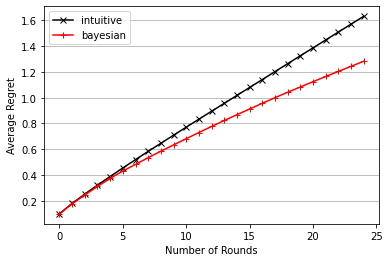
\includegraphics[width = 0.5\textwidth]{part2.png}
            \caption{The cumulative regret of the intuitive policy and the optimal policy with actual theta at 0.6, 1. The actual theta value is deliberately set so that the result is more obvious. The intuitive policy has a large probability of sticking with arm 1, since arm 1 already has a not bad probability of yielding a reward. This is also in accord with the example we give for when the intuitive policy is not optimal. As we can see, the optimal policy has an obviously better performance in this case.}
            \label{fig4}
        \end{figure}
        \begin{figure}[htp]
            \centering
            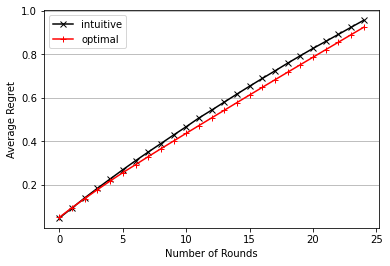
\includegraphics[width = 0.5\textwidth]{part2(2).png}
            \caption{The cumulative regret of the intuitive policy and the optimal policy with actual theta at 0.2, 0.3. This test shows that even when the intuitive policy behaves very good, the optimal policy gives similar good results.}
            \label{fig5}
        \end{figure}
        \begin{figure}[htp]
            \centering
            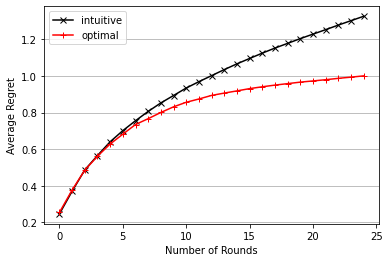
\includegraphics[width = 0.5\textwidth]{part2(3).png}
            \caption{The cumulative regret of the intuitive policy and the optimal policy with actual theta at 0.8, 0.3. This test shows that even when the intuitive policy behaves quite well, the optimal policy still improves the overall regret.}
            \label{fig6}
        \end{figure}
        \begin{figure}[htp]
            \centering
            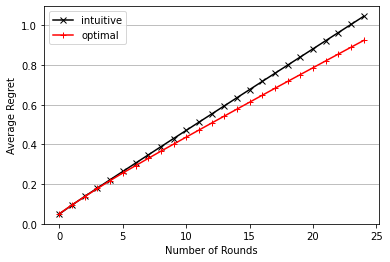
\includegraphics[width = 0.5\textwidth]{part2(4).png}
            \caption{The cumulative regret of the intuitive policy and the optimal policy with actual theta at 0.8, 0.9. This test shows that the counter example we gave for the intuitive policy in 2 is correct.}
            \label{fig7}
        \end{figure}
    \end{enumerate}
\end{homeworkProblem}
\pagebreak


\begin{thebibliography}{99}

\bibitem{ref1} https://zhuanlan.zhihu.com/p/84140092, https://zhuanlan.zhihu.com/p/84200578, \\https://zhuanlan.zhihu.com/p/84338172
\bibitem{ref2} Rahul Singh, Fang Liu, Yin Sun, Ness Shroff, \textsl{Multi-Armed Bandits with Dependent Arms}
\bibitem{ref3} Samarth Gupta, Shreyas Chaudhari, Gauri Joshi, Osman Yağan, \textsl{Multi-Armed Bandits with Correlated Arms}
\bibitem{ref4} S. Agrawal and N. Goyal, “Further optimal regret bounds for Thompson sampling,” in \textsl{Artificial Intelligence and Statistics}, pp. 99-107, 2013.
\bibitem{ref5} Richard S. Sutton and Andrew G. Barto, \textsl{Reinforcement Learning: An Introduction}
\bibitem{ref6} Lucas Descause, \textsl{Reinforcement Learning with Function Approximation in Continuing Tasks: Discounted Return or Average Reward?}

\end{thebibliography}

\end{document}